\begin{figure*}
	\centering
	\begin{adjustbox}{width=\textwidth}
		\begin{tikzpicture}[auto]
			\tikzstyle{terminal} = [rectangle, draw, text width=5em, text centered, minimum height=4em]
			\tikzstyle{block} = [rectangle, draw, fill=gray!20, text width=6em, text centered, rounded corners, minimum height=4em]
			\tikzstyle{line} = [draw, -latex']
			\tikzstyle{sum} = [circle, draw]

			\node[inner sep=0pt] (bertrand) {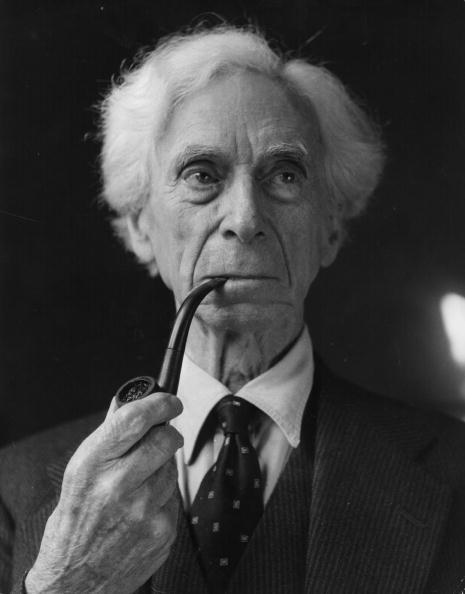
\includegraphics[width=.15\textwidth]{figures/background/bertrand/bertrand.png}};
			\node [above = of bertrand] (scene) {Scene};

			\node[sum, right = of bertrand] (sum1) {\(+\)};
			\node [block, below = of sum1] (atmo-noise) {Atmospheric noise};

			\node [block, right = of sum1] (motion) {Translation, Rotation, Aspect};
			\node [above = of motion] {Motion};

			\node [inner sep=0pt, right = of motion] (motion-output) {};

			\node[inner sep=0pt, below = of motion-output] (bertrand-motion) {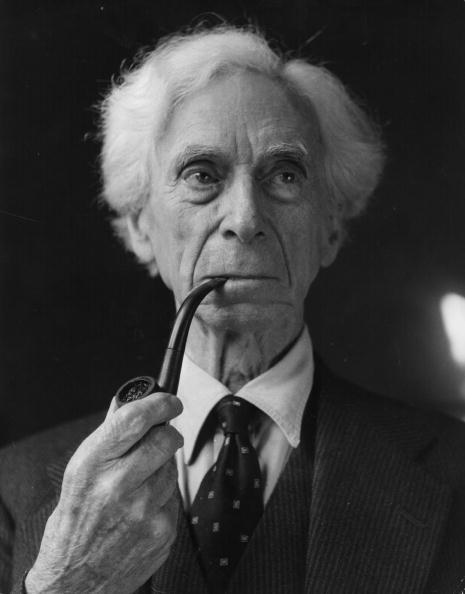
\includegraphics[width=.15\textwidth]{figures/background/bertrand/bertrand.png}};
			\node[inner sep=0pt, below = of motion-output, xshift=2mm, yshift=-2mm] {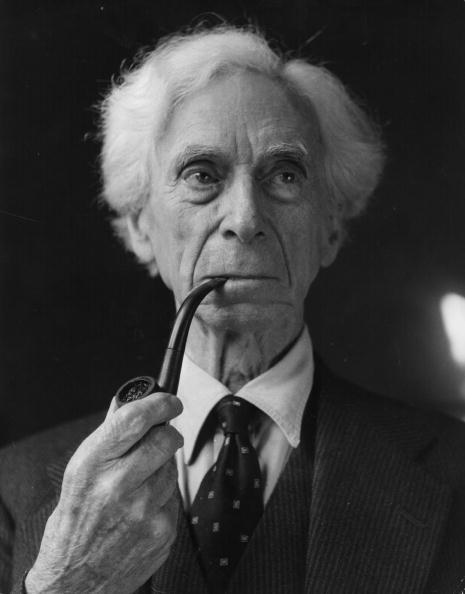
\includegraphics[width=.15\textwidth]{figures/background/bertrand/bertrand.png}};
			\node[inner sep=0pt, below = of motion-output, xshift=4mm, yshift=-4mm] {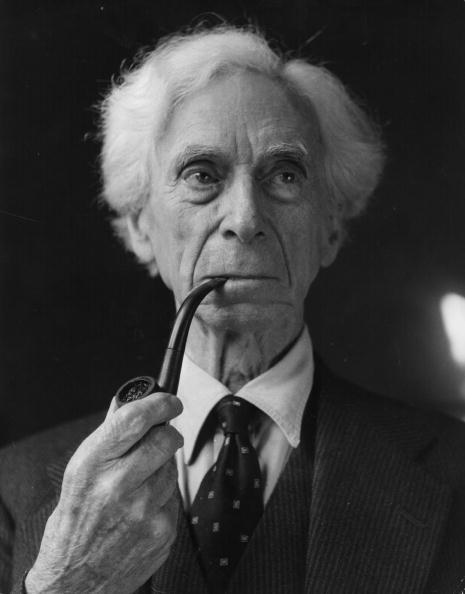
\includegraphics[width=.15\textwidth]{figures/background/bertrand/bertrand.png}};
			\node[inner sep=0pt, below = of motion-output, xshift=6mm, yshift=-6mm] {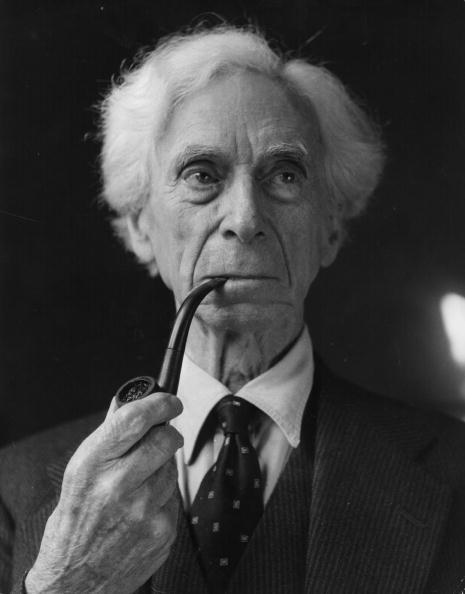
\includegraphics[width=.15\textwidth]{figures/background/bertrand/bertrand.png}};

			\node [block, right = of motion-output] (blur) {Optical, Motion};
			\node [above = of blur] {Blur};
			\node [inner sep=0pt, right = of blur] (blur-output) {};

			\node[inner sep=0pt, below = of blur-output] (bertrand-blur) {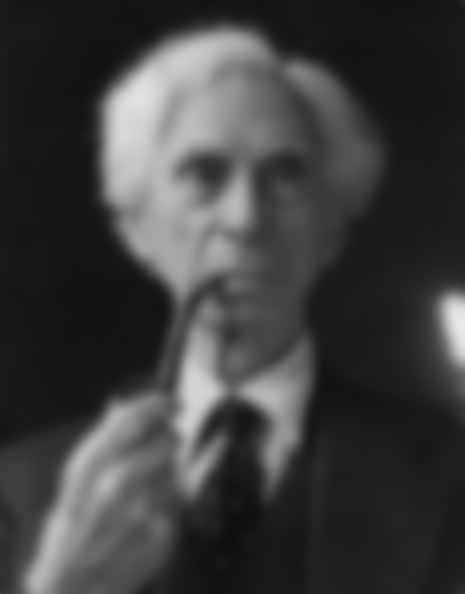
\includegraphics[width=.15\textwidth]{figures/background/bertrand/bertrand-blur.png}};
			\node[inner sep=0pt, below = of blur-output, xshift=2mm, yshift=-2mm] {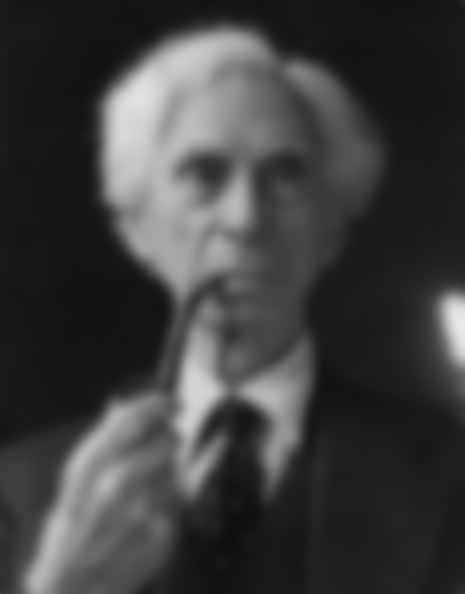
\includegraphics[width=.15\textwidth]{figures/background/bertrand/bertrand-blur.png}};
			\node[inner sep=0pt, below = of blur-output, xshift=4mm, yshift=-4mm] {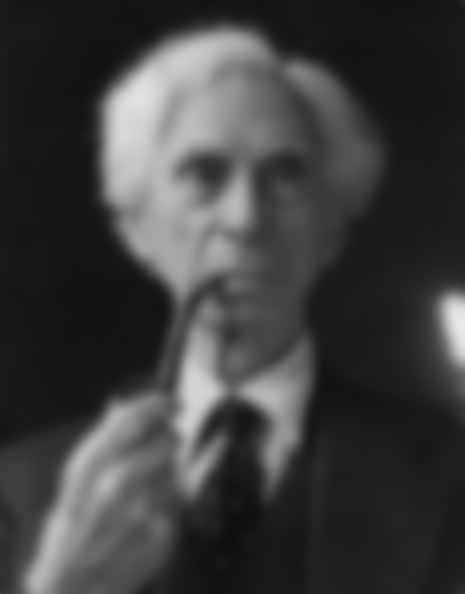
\includegraphics[width=.15\textwidth]{figures/background/bertrand/bertrand-blur.png}};
			\node[inner sep=0pt, below = of blur-output, xshift=6mm, yshift=-6mm] {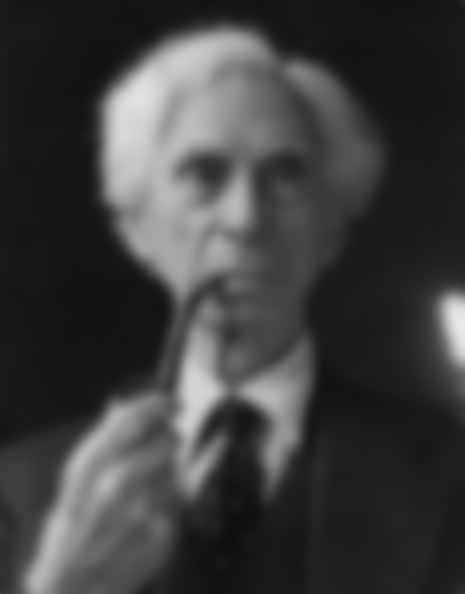
\includegraphics[width=.15\textwidth]{figures/background/bertrand/bertrand-blur.png}};

			\node[block, right = of blur-output] (downsample) {Quantization, Pixel-binning};
			\node [above = of downsample] {Down-sampling};

			\node[sum, right = of downsample] (sum2) {\(+\)};
			\node [block, below = of sum2] (sensor-noise) {Sensor noise};

			\node[inner sep=0pt, right = of sum2] (bertrand-blur-noise) {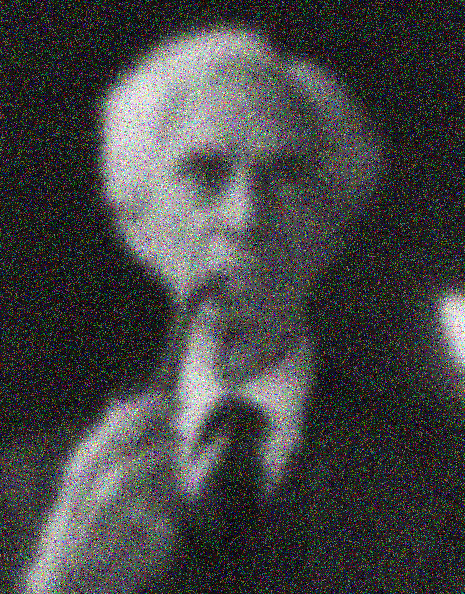
\includegraphics[width=.1\textwidth]{figures/background/bertrand/bertrand-blur-noise.png}};
			\node[inner sep=0pt, right = of sum2, xshift=2mm, yshift=-2mm] {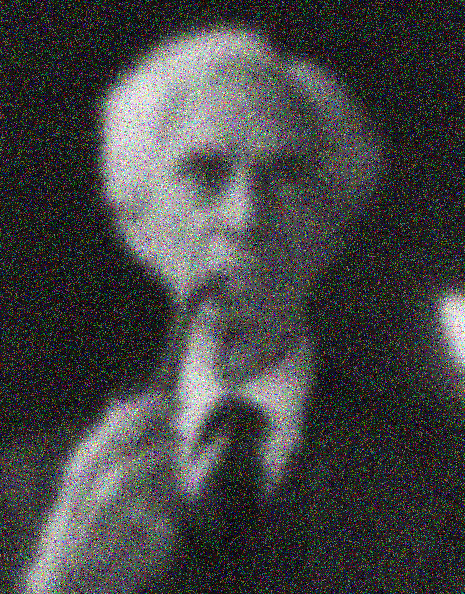
\includegraphics[width=.1\textwidth]{figures/background/bertrand/bertrand-blur-noise.png}};
			\node[inner sep=0pt, right = of sum2, xshift=4mm, yshift=-4mm] {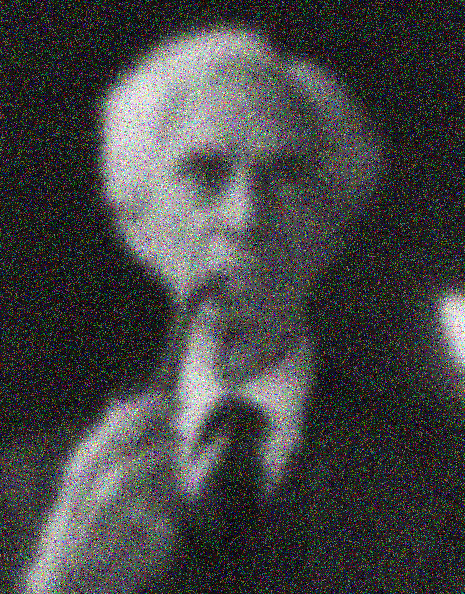
\includegraphics[width=.1\textwidth]{figures/background/bertrand/bertrand-blur-noise.png}};
			\node[inner sep=0pt, right = of sum2, xshift=6mm, yshift=-6mm] {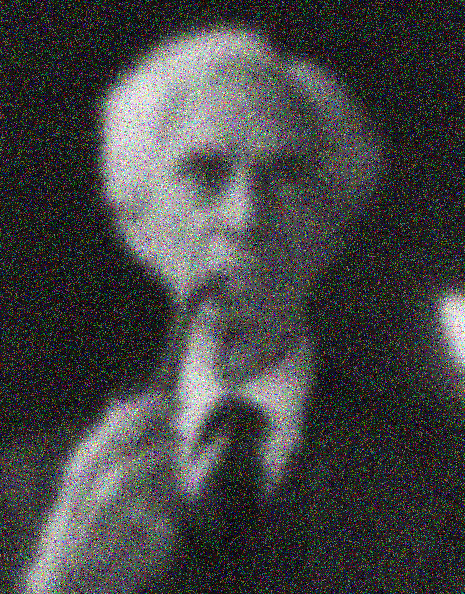
\includegraphics[width=.1\textwidth]{figures/background/bertrand/bertrand-blur-noise.png}};
			\node [above = of bertrand-blur-noise, text width=5em] (lr-output) {Low-resolution images};

			\draw[-] (bertrand) edge (sum1);
			\draw[->] (sum1) edge (motion);
			\draw[->] (atmo-noise) edge (sum1);

			\draw[->] (motion) edge (blur);
			\draw[->] (motion-output) edge (bertrand-motion);

			\draw[->] (blur) edge (downsample);
			\draw[->] (blur-output) edge (bertrand-blur);
			\draw[->] (sensor-noise) edge (sum2);
			\draw[-] (downsample) edge (sum2);
			\draw[->] (sum2) edge (bertrand-blur-noise);
		\end{tikzpicture}
	\end{adjustbox}
	\caption{The imaging model illustrating the relationship between a scene and final low-resolution images due to noise, motion, blur, and sampling.}
	\label{fig:bertrand}
\end{figure*}
